%Este trabalho está licenciado sob a Licença Atribuição-CompartilhaIgual 4.0 Internacional Creative Commons. Para visualizar uma cópia desta licença, visite http://creativecommons.org/licenses/by-sa/4.0/deed.pt_BR ou mande uma carta para Creative Commons, PO Box 1866, Mountain View, CA 94042, USA.

\chapter{Problema de Valor de Contorno}\label{cap_pvc}
\thispagestyle{fancy}

Neste capítulo, \hl{estudamos métodos numéricos para resolver \emph{Problemas de Valores de Contorno}} da forma
\begin{subequations}\hleq
  \begin{align}
    &u'' = f(x, u, u'), ~a < x < b,\\
    &\eta_1 u'(a) + \theta_1 u(b) = g_1\\
    &\eta_2 u'(b) + \theta_2 u(b) = g_2
\end{align}
\end{subequations}
onde a incógnita é $u = u(x)$ com dada $f = f(x, u, u')$ e dados parâmetros $\eta_1$, $\theta_1$ (não simultaneamente nulos), $\eta_2$, $\theta_2$ (não simultaneamente nulos), $g1$ e $g2$.

\section{Método de Diferenças Finitas}\label{cap_pvc_sec_mdf}

Consideramos o seguinte Problema Linear de Valor de Contorno (PVC)
\begin{subequations}\label{cap_pvc_sec_mdf:eq:pvc}\hleq
  \begin{align}
    &u'' + \alpha(x) u' + \beta(x) u = f(x), ~a < x < b, \label{cap_pvc_sec_mdf:eq:pvc_eq}\\
    &u(a) = g, \label{cap_pvc_sec_mdf:eq:pvc_bc1}\\
    &u(b) = h. \label{cap_pvc_sec_mdf:eq:pvc_bc2}
  \end{align}
\end{subequations}
onde a incógnita é $u = u(x)$ com dada fonte $f = f(x)$ e dados parâmetros $g$ e $h$.

\hl{A aproximação pelo \emph{Método de Diferenças Finitas} (MDF) de {\eqref{cap_pvc_sec_mdf:eq:pvc_eq}}-{\eqref{cap_pvc_sec_mdf:eq:pvc_bc2}} surge da substituição das derivadas por Fórmulas de Diferenças Finitas}. De forma geral, o método pode ser dividido em três etapas: 1. discretização do domínio, 2. discretização das equações, 3. resolução do problema discreto.

\begin{flushleft}
  \emph{1. Discretização do Domínio}
\end{flushleft}

\hl{A \emph{discretização do domínio} é seu particionamento em \emph{subintervalos} (\emph{células} computacionais) e \emph{pontos} (\emph{nodos} computacionais)}. Por simplicidade, vamos considerar apenas o caso de um particionamento uniforme. Particionamos o domínio $D = [a, b]$ em $n$ de subintervalos de \emph{tamanho de malha}
\begin{equation}\hleq
  h = \frac{b-a}{n},
\end{equation}
e os nodos da partição podem ser indexados da seguinte forma
\begin{equation}\hleq
  x_i = a + (i-1)h,
\end{equation}
com $i = 1, 2, 3, \dotsc, n+1$.

\begin{flushleft}
  {\bf 2. Discretização das Equações}
\end{flushleft}

Começando por \eqref{cap_pvc_sec_mdf:eq:pvc_eq}, em um nodo \hl{$x=x_i$, $i=2, 3, \dotsc, n$}, temos
\begin{equation}\label{cap_pvc_sec_mdf:eq:pvc_eq_no_ponto}
  u''(x_i) + \alpha(x_i) u'(x_i) + \beta(x_i) u(x_i) = f(x_i).
\end{equation}
Podemos substituir a segunda derivada de $u$ pela \emph{fórmula de diferenças finitas} central de ordem $h^2$
\begin{equation}
  u''(x_i) = \underbrace{\frac{u(x_i-h) - 2u(x_i) + u(x_i+h)}{h^2}}_{D^2_{0,h^2}u(x_i)} + O(h^2).
\end{equation}
A primeira derivada de $u$ também pode ser substituída pela fórmula de diferenças finitas central de ordem $h^2$
\begin{equation}
  u'(x_i) = \underbrace{\frac{u(x_i+h)-u(x_i-h)}{2h}}_{D_{0,h^2}u(x_i)} + O(h^2).
\end{equation}

Agora, denotando \hl{$u_i \approx u(x_i)$}, temos $u_{i-1}\approx u(x_i-h)$ e $u_{i+1}\approx u(x_i+h)$. Substituindo as derivadas pelas fórmulas de diferenças finitas, temos de \eqref{cap_pvc_sec_mdf:eq:pvc_eq_no_ponto} que
\begin{equation}
  \begin{aligned}
    &\left(\frac{u_{i-1}-2u_i+u_{i+1}}{h^2}\right) + \alpha(x_i)\left(\frac{u_{i+1}-u_{i-1}}{2h}\right) \\
    &\quad + \beta(x_i)u_i + O(h^2) = f(x_i),
  \end{aligned}
\end{equation}
Rearranjando os termos e desconsiderando o termo do erro de truncamento, obtemos o seguinte sistema de equações lineares
\begin{equation}\label{cap_pvc_sec_mdf:eq:pvc_mdf_sis1}
  \begin{aligned}
    &\left(\frac{1}{h^2}-\frac{\alpha_i}{2h}\right)u_{i-1} + \left(\beta_i - \frac{2}{h^2}\right)u_i\\
    &\quad + \left(\frac{1}{h^2}+\frac{\alpha_i}{2h}\right)u_{i+1} = f_i, 
  \end{aligned}
\end{equation}
onde, usamos a notação $\alpha_i = \alpha(x_i)$, $\beta_i = \beta(x_i)$ e $f_i = f(x_i)$.

Observamos que este sistema consiste em $n-1$ equações envolvendo as $n+1$ incógnitas $u_i$, $i=1, 2, \dotsc, n+1$. Para fechá-lo, usamos as condições de contorno. De \eqref{cap_pvc_sec_mdf:eq:pvc_bc1}, temos
\begin{equation}\label{cap_pvc_sec_mdf:eq:pvc_mdf_sis0}
  u_1 = g
\end{equation}
e de \eqref{cap_pvc_sec_mdf:eq:pvc_bc2} temos
\begin{equation}\label{cap_pvc_sec_mdf:eq:pvc_mdf_sis2}
  u_{n+1} = h,
\end{equation}
lembrando que $u_0\approx u(x_0)$ e $u_n\approx u(x_n)$.

Por fim, as equações \eqref{cap_pvc_sec_mdf:eq:pvc_mdf_sis1}-\eqref{cap_pvc_sec_mdf:eq:pvc_mdf_sis2} formam o seguinte \emph{problema discretizado}
\begin{subequations}\label{cap_pvc_sec_mdf:eq:pd}\hleq
  \begin{align}
    &u_1 = g,\\
    &~\nonumber\\
    &\left(\frac{1}{h^2}-\frac{\alpha_i}{2h}\right)u_{i-1} + \left(\beta_i - \frac{2}{h^2}\right)u_i \nonumber\\
    &\quad + \left(\frac{1}{h^2}+\frac{\alpha_i}{2h}\right)u_{i+1} = f_i,\\
    &~\nonumber\\
    &u_{n+1} = h,
  \end{align}
\end{subequations}
para $i = 2, 3, \dotsc, n$.

\begin{flushleft}
  {\bf 3. Resolução do problema discreto}
\end{flushleft}

\hl{O problema discreto {\eqref{cap_pvc_sec_mdf:eq:pd}} consiste em um sistema linear de $n+1$ equações com $n+1$ incógnitas}. Na forma matricial temos
\begin{equation}\eqref{cap_pvc_sec_mdf:eq:sis_mdf}
  A\pmb{u} = \pmb{b}
\end{equation}
onde $\pmb{u} = (u_1, u_2, \dotsc, u_{n+1})$ é o vetor das incógnitas, $\pmb{b} = (g, f_2, f_3, \dotsc, f_{n}, h)$. A matriz dos coeficientes é  $A = [a_{i,j}]_{i,j=1}^{n+1,n+1}$ e seus elementos não nulos são
\begin{align}
  &a_{1,1} = 1,
  & ~ \nonumber \\
  &a_{i,i-1} = \frac{1}{h^2}-\frac{\alpha_i}{2h},\\
  &a_{i,i} = \beta_i - \frac{2}{h^2}, \\
  &a_{i,i+1} = \frac{1}{h^2}+\frac{\alpha_i}{2h},\\
  & ~ \nonumber \\
  &a_{n+1,n+1} = 1,
\end{align}
para $i = 2, 3, \dotsc, n$.

\hl{A resolução do sistema discreto se resume, a resolver o sistema $A\pmb{u} = \pmb{b}$}, o que pode ser feito por qualquer método numérico apropriado.

\begin{ex}\label{cap_pvc_sec_mdf:ex:pvc_mdf_1}
  Consideramos o seguinte PVC
  \begin{align}
    &-u'' = \pi^2\sen(\pi x), ~0 < x < 1,\\
    &u(0) = 0,\\
    &u(1) = 0.
  \end{align}

\begin{figure}[h!]
  \centering
  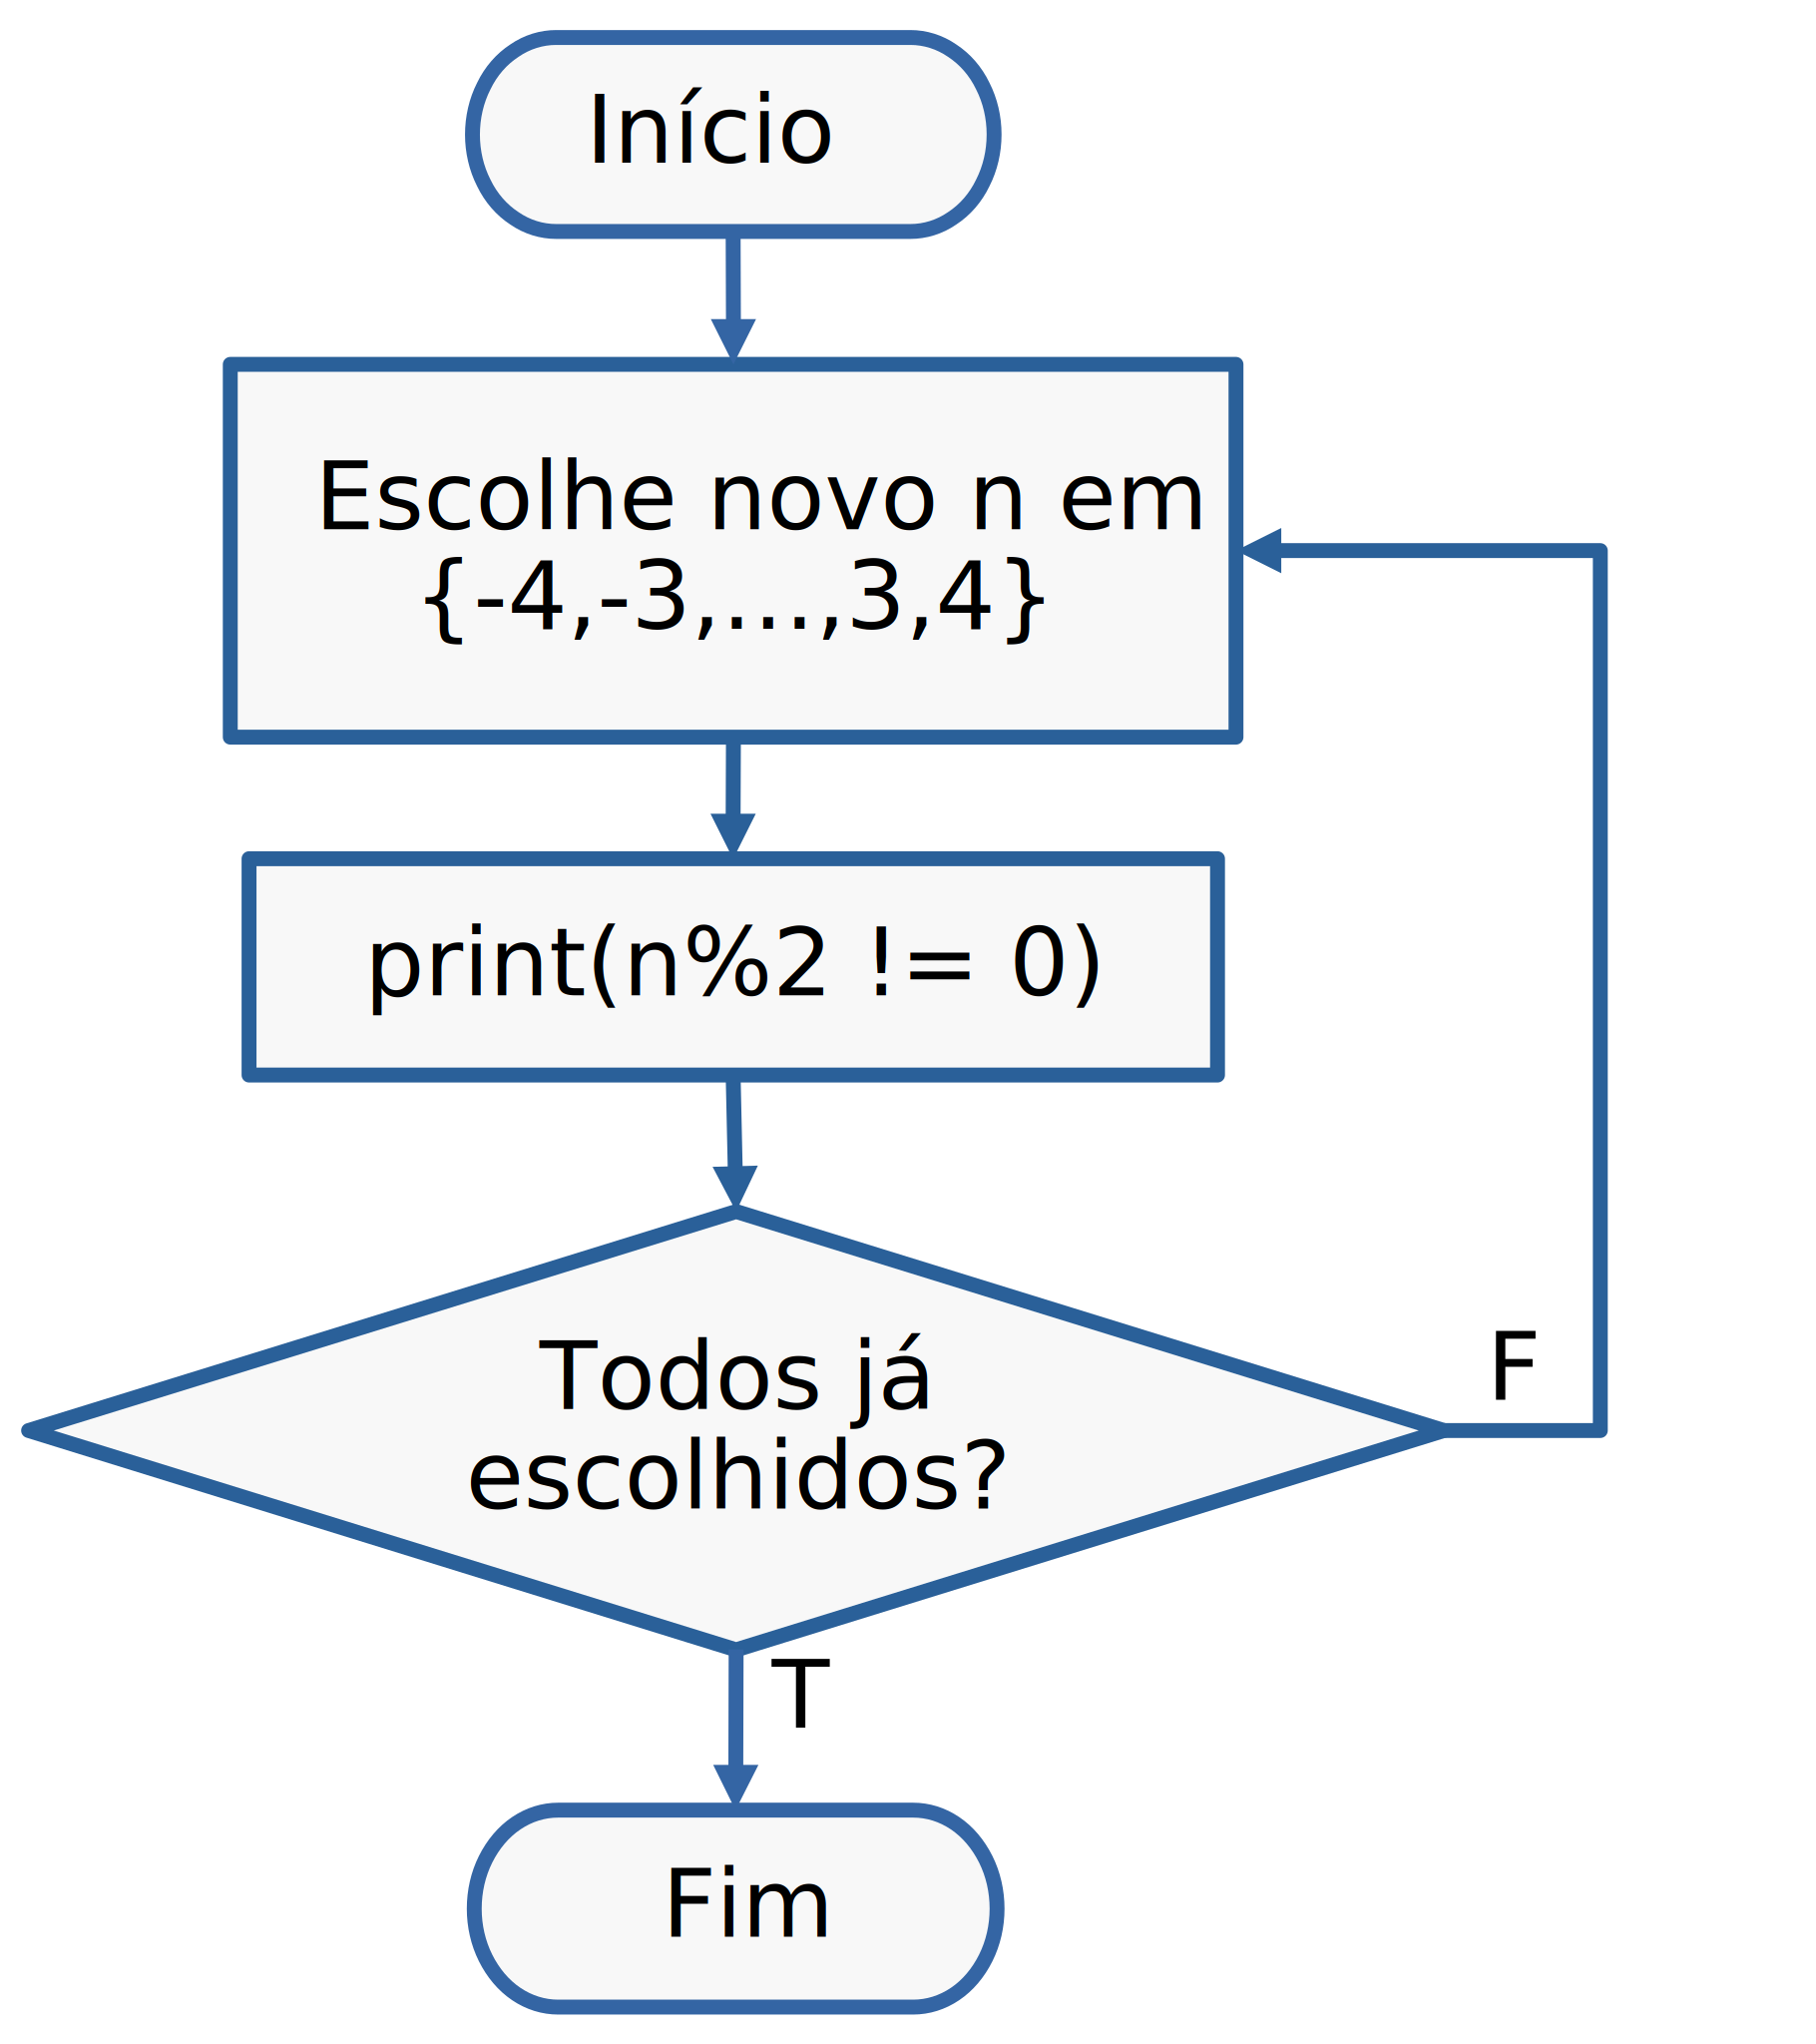
\includegraphics[width=0.8\textwidth]{./cap_pvc/dados/fig_mdf/fig}
  \caption{Resultado referente ao Exemplo~\ref{cap_pvc_sec_mdf:ex:pvc_mdf_1}.}
  \label{cap_pvc_sec_mdf:fig:ex_pvc_mdf_1}
\end{figure}

A solução analítica deste problema é $u(x) = \sen(\pi x)$. Usando o MDF como acima, encontramos o problema discreto
\begin{subequations}
  \begin{align}
    u_1 &= 0,\\
    -\frac{1}{h^2}u_{i-1} + \frac{2}{h^2}u_i - \frac{1}{h^2}u_{i+1} &= \pi^2\sen(\pi x_i),\\
    u_{n+1} &= 0,
  \end{align}
\end{subequations}
com tamanho de malha $h=1/n$ e nodos $x_i = (i-1)h$ indexados por $i = 1, 2, \dotsc, n+1$.

\begin{table}[h!]
  \centering
  \caption{Resultados referentes ao Exemplo~\ref{cap_pvc_sec_mdf:ex:pvc_mdf_1}.}
  \begin{tabular}{l|c}\toprule
    $h$ & $\|\tilde{u} - u\|_{L^2}$ \\\midrule
    $1.0\e-1$ & $1.8\e-2$\\
    $5.0\e-2$ & $6.5\e-3$\\
    $2.5\e-2$ & $2.3\e-3$\\
    $1.0\e-3$ & $5.8\e-4$\\\bottomrule
  \end{tabular}
  \label{cap_pvc_sec_mdf:tab:ex_pvc_mdf_1}
\end{table}

Resolvendo este sistema com $h=10^{-1}$ obtemos a solução numérica apresentada na Figura~\ref{cap_pvc_sec_mdf:fig:ex_pvc_mdf_1}. Ainda, na Tabela~\ref{cap_pvc_sec_mdf:tab:ex_pvc_mdf_1} temos a comparação na norma $L^2$ da solução numérica $\tilde{\pmb{u}}$ com a solução analítica $\pmb{u} = (u(x_i))_{i=1}^{n+1}$ para diferentes escolhas de $h$.

\begin{lstlisting}
import numpy as np
import numpy.linalg as npla
import matplotlib.pyplot as plt

plt.rcParams.update({
     "text.usetex": True,
     "font.family": "serif",
     "font.size": 14
     })


# malha
n = 10
h = 1./n
xx = np.linspace(0., 1., n+1)

# fonte
def f(x):
    return np.pi**2*np.sin(np.pi*x)

# prob discreto
A = np.zeros((n+1, n+1))
b = np.empty(n+1)

# c.c. x = 0.
A[0,0] = 1.
b[0] = 0.

# pts internos
for i in range(1,n):
    A[i,i-1] = -1./h**2
    A[i,i] = 2./h**2
    A[i,i+1] = -1./h**2
    b[i] = f(xx[i])

# c.c. x = 1.
A[n,n] = 1.
b[n] = 0.

# resol
u = npla.solve(A, b)
\end{lstlisting}
\end{ex}

\subsection*{Exercícios}

\begin{exer}
  Considere o PVC
  \begin{align}
    &-u'' = \pi^2\cos(\pi x), ~0 < x < 1,\\
    &u(0) = 1,\\
    &u(1) = -1.
  \end{align}
  A solução analítica deste problema é $u(x) = \cos(\pi x)$. Use o MDF para computar aproximações numéricas $\tilde{\pmb{u}}_h$ com tamanhos de malha $h=10^{-1}, 10^{-2}, 10^{-3}, 10^{-4}$ e verifique o erro absoluto $\varepsilon_{\text{abs}} := \|\tilde{\pmb{u}}_h - \pmb{u}\|$.
\end{exer}
\begin{resp}
  \begin{tabular}{l|c}\toprule
    $h$ & $\|\tilde{u} - u\|_{L^2}$ \\\midrule
    $10^{-1}$ & $3.9\e-3$\\
    $10^{-2}$ & $1.2\e-4$\\
    $10^{-3}$ & $3.9\e-6$\\
    $10^{-4}$ & $1.2\e-7$\\\bottomrule
  \end{tabular}  
\end{resp}

\begin{exer}
  Considere o PVC
  \begin{align}
    &-u'' = 1, ~-1 < x < 1,\\
    &u(-1) = 0,\\
    &u(1) = 0.
  \end{align}
  A solução analítica deste problema é $u(x) = 1-x^2$. Use o MDF com $n=20$ subintervalos na malha e verifique o erro absoluto $\varepsilon_{\text{abs}} := \|\tilde{\pmb{u}}_h - \pmb{u}\|$. Por que o erro está próximo precisão de máquina? Justifique sua resposta.
\end{exer}
\begin{resp}
  $\varepsilon_{\text{abs}} = 3.1\e-14$.
\end{resp}

\begin{exer}
Considere o seguinte PVC
\begin{subequations}
  \begin{align}
    &-u'' + u' = f(x), ~-1 < x < 1,\\
    &u(-1) = 0,\\
    &u'(1) =0,
  \end{align}
\end{subequations}
onde
\begin{equation}
  f(x) = \left\{
    \begin{array}{ll}
      1 &, x\leq 0\\
      0 &, x>0
    \end{array}
  \right.
\end{equation}
\end{exer}
Use uma aproximação adequada pelo método de diferenças finitas para obter o valor aproximado de $u(0)$ com precisão de $2$ dígitos significativos.
\begin{resp}
  $7,2\E-1$
\end{resp}

\begin{exer}
  Considere o PVC
  \begin{align}
    &-u'' = \pi^2\cos(\pi x), ~0 < x < 1,\\
    &u(0) = 1,\\
    &u'(1) = 0.
  \end{align}
  A solução analítica deste problema é $u(x) = \cos(\pi x)$. Aplique o MDF para computar aproximações numéricas usando a:
  \begin{enumerate}[a)]
  \item fórmula de diferenças finitas $D_{-,h}u(x)$ no contorno $x=1$.
  \item fórmula de diferenças finitas $D_{-,h^2}u(x)$ no contorno $x=1$.
  \end{enumerate}
  Quais das duas produz o resultado mais preciso? Justifique sua resposta.
\end{exer}
\begin{resp}
  b) resultado mais preciso.
\end{resp}


